\chapter{Extended Literature Review}
\label{chap:extended_literature_review}
This extended chapter reviews techniques to enhance semantic segmentation models' performance. The following summaries were created during the project's goal-finding process aiming to offer an in-depth perspective on the topic. The techniques discussed in this chapter are being applied to various tasks, but the focus of the cited papers is specifically on their use in semantic segmentation. The methods are categorized to facilitate understanding and comparison. Each technique is introduced with a general overview or survey, followed by a chronological presentation of specific approaches, with the most recent techniques being presented first.
\begin{itemize}[noitemsep]
    \item Data Augmentation
    \item Multi-scale Processing
    \item Ensemble Learning
    \item Transfer Learning
    \item Weakly-supervised Learning
    \item Active Learning
    \item Semi-supervised Learning
    \item Domain Adaption
    \item Post-processing
    \item Multi-task Learning
    \item Attention Mechanisms
    \item Reinforcement Learning
\end{itemize}
\section{Data Augmentation}
\squote{A survey on image data augmentation for deep learning} \cite{shorten2019survey} from 2019 provides an extensive study for data augmentation. \textit{Data augmentation} is a technique used to improve deep learning models by enhancing the size and quality of training datasets. It invovles a variety of techniques, including geometric transformations \cite{taylor2018improving}, color space augmentations, and neural style transfer \cite{shorten2019survey}. The paper also covers other aspects of data augmentation, such as test-time augmentation, resolution impact, and curriculum learning. Data augmentation aims to increase model performance and expand limited datasets to be more similar to large datasets.

\squote{A Simple Baseline for Semi-Supervised Semantic Segmentation With Strong Data Augmentation} \cite{Yuan_2021_ICCV} from 2021 presents a semi-supervised model with strong data augmentation. Their approach is specific for semi-supervised models where many unlabeled training samples are added to the labeled dataset. To balance the disadvantage of batch normalization \footnote{Batch normalization normalizes activations in hidden layers of deep neural networks and is supposed to improve accuracy and speed up training. While networks without batch normalization tend to diverge with significant learning rates, batch normalization can avoid this problem as the activations are corrected to be zero-mean and of unit standard deviation, enabling more significant gradient steps, yielding faster convergence and helping to bypass local minima \cite{NEURIPS2018_36072923}} for semi-supervised models (distribution mismatch), they propose a distribution specific batch normalization and forward strongly augmented and weakly-augmented data with different batch statistics. Their method achieves state-of-the-art results in the semi-supervised settings on CityScapes \cite{cordts2016cityscapes} and Pascal VOC \cite{hoiem2009pascal} datasets.

\squote{Optimizing Data Augmentation for Semantic Segmentation on Small-Scale Dataset} \cite{10.1145/3341016.3341020} from 2019 aims to optimize data augmentation methods for semantic segmentation. The authors summarize important methods in two groups and call them global and local data augmentation. Global data augmentation refers to augmenting images, while local augmentation is specific to objects within the image. They combine different data augmentation techniques and achieve the best results with compression, cropping, and local shift. The authors claim to improve the mean \ac{IoU} from 73.3\% to 91.3\%. The model was trained on a small custom dataset built from scratch for sheep body recognition and segmentation.

\squote{Improving Data Augmentation for Medical Image Segmentation} \cite{EatonRosen2018ImprovingDA} from 2018, evaluates an augmentation method for medical images, called \squote{mixup} where each sample label pair is a linear combination of two sample label pairs calculated as:
\begin{equation}
    x_{mixup}=\lambda x_i +(1-\lambda) x_j
\end{equation}
\begin{equation}
    y_{mixup}=\lambda y_i +(1-\lambda) y_j
\end{equation}
where $\lambda \ in [0,1]$ and drawn from $\lambda \sim \beta(\alpha,\alpha)$ for $\alpha \in (0,\infty)$ according to a Beta distribution \footnote{The Beta distribution is a continuous probability distribution defined on the interval $[0, 1]$ and parameterized by two positive shape parameters, $\alpha$, and $\beta$. It helps model random variables with a fixed range related to proportions, percentages, or probabilities. The Beta distribution is a member of the exponential family and is conjugate to the Bernoulli and binomial distributions, making it convenient for Bayesian inference.\cite{doi:10.1080/0266476042000214501}\cite{gelman2013bayesian}}. This method has been shown to improve performance on several machine-learning tasks. The authors additionally implemented a new method called \squote{mixmatch}, a variant from \squote{mixup} by considering class prevalence. Both methods are then used to train the BraTS \cite{bakas2018identifying} dataset, outperforming training without these methods.

\squote{Large Scale Labelled Video Data Augmentation for Semantic Segmentation in Driving Scenarios} \cite{Budvytis_2017_ICCV} from 2017, proposes a simplified version of the label propagation algorithm presented by \cite{budvytis2011semi}. \textit{Label propagation} is an augmentation technique that labels unlabeled data points based on their similarity to labeled data points. Thus, label propagation is commonly used in semi-supervised learning, where a dataset contains a lot of unlabeled and few labeled data points. The authors apply their algorithm on the CityScapes \cite{cordts2016cityscapes} and CamVid \cite{brostow2009semantic} dataset observing a significant increase in performance.

\section{Improved Feature Extraction}
\textit{Feature extraction} is a process used to reduce the dimensionality of data and extract meaningful features from it. It differs from feature selection, which involves identifying a subset of the original dimensions containing the most information and discarding the rest. In contrast, feature extraction involves finding a new set of dimensions that are combinations of the original dimensions and are more effective at representing the data \cite{alpaydin2020introduction}.

In traditional machine learning techniques, feature extraction is typically performed using techniques such as principal component analysis \cite{abdi2010principal} or linear discriminant analysis \cite{balakrishnama1998linear}. However, feature extraction is usually performed automatically using convolutional layers in deep learning, particularly with \acp{CNN}. Early layers in a \acp{CNN} might extract low-level features such as edges and corners, while later layers extract higher-level features such as objects or patterns.\cite{hijazi2015using}

Enhancing feature extraction in the context of semantic segmentation means improving the ability of the convolutional layers in the deep learning architecture to extract relevant and useful features for the current task. The following paragraphs discuss various approaches to designing the \acp{CNN} architecture and filters to optimize the quality and effectiveness of the extracted features to improve the model's performance.

\begin{figure}[H]%[htbp]
    \centering
    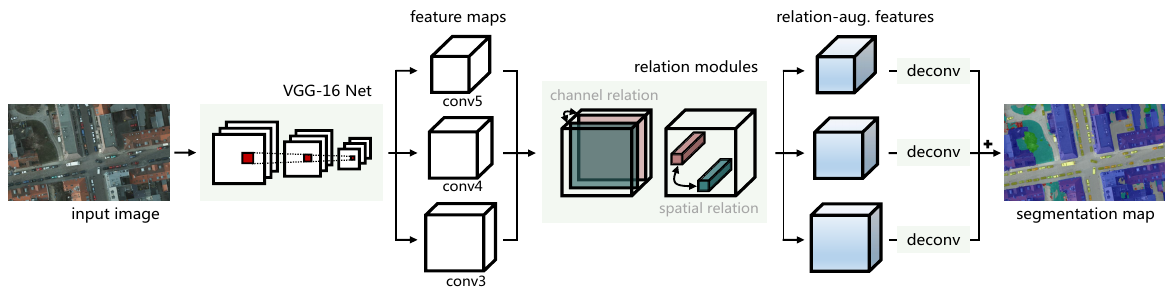
\includegraphics[width=\imgWidthXL]{images/relation_matters_network.png}
    \caption[Relation focused architecture]{\acf{CNN} architecture featuring a channel and spatial relation module, as shown in the image from \cite{9076866}.}
    \label{relation_matters_network}
\end{figure}

\squote{Relation Matters: Relational Context-Aware Fully Convolutional Network for Semantic Segmentation of High-Resolution Aerial Images} \cite{9076866} from 2020 proposes an innovative approach to enhance feature extraction for semantic segmentation of aerial images using a \ac{CNN}. See \figref{relation_matters_network} for further information on the architecture. Their goal is to capture both long-range spatial relationships and channel-wise information, which helps to address challenges such as visual ambiguities\footnote{Visual ambiguities occur when visual information is incomplete, noisy or has multiple interpretations.\cite{BibEntry2023MarAmbiguity}\cite{boring1930new}\cite{kanizsa1976subjective}} and appearance variations. The effectiveness of this method is demonstrated through ablation studies, which show that the network can perform both channel and spatial reasoning and effectively process relational context. The results of this study suggest that this approach may be a valuable tool for improving semantic segmentation in aerial imagery.

\squote{Context Encoding for Semantic Segmentation} \cite{https://doi.org/10.48550/arxiv.1803.08904} from 2018 introduces the \acf{CEM}  for semantic segmentation using a \acf{FCN}. The module captures the semantic context of scenes and selectively highlights class-dependent feature maps, significantly improving semantic segmentation results with only marginal extra computation cost. See \figref{context_encoding_module} for further details on the architecture. The authors achieved new state-of-the-art results on PASCAL-Context \cite{everingham2015pascal} and PASCAL VOC 2012 \cite{pascal-voc-2012} datasets and also explored the module's impact on improving feature representation for image classification on CIFAR-10 \cite{cifar10dataset} dataset.

\begin{figure}[H]%[htbp]
    \centering
    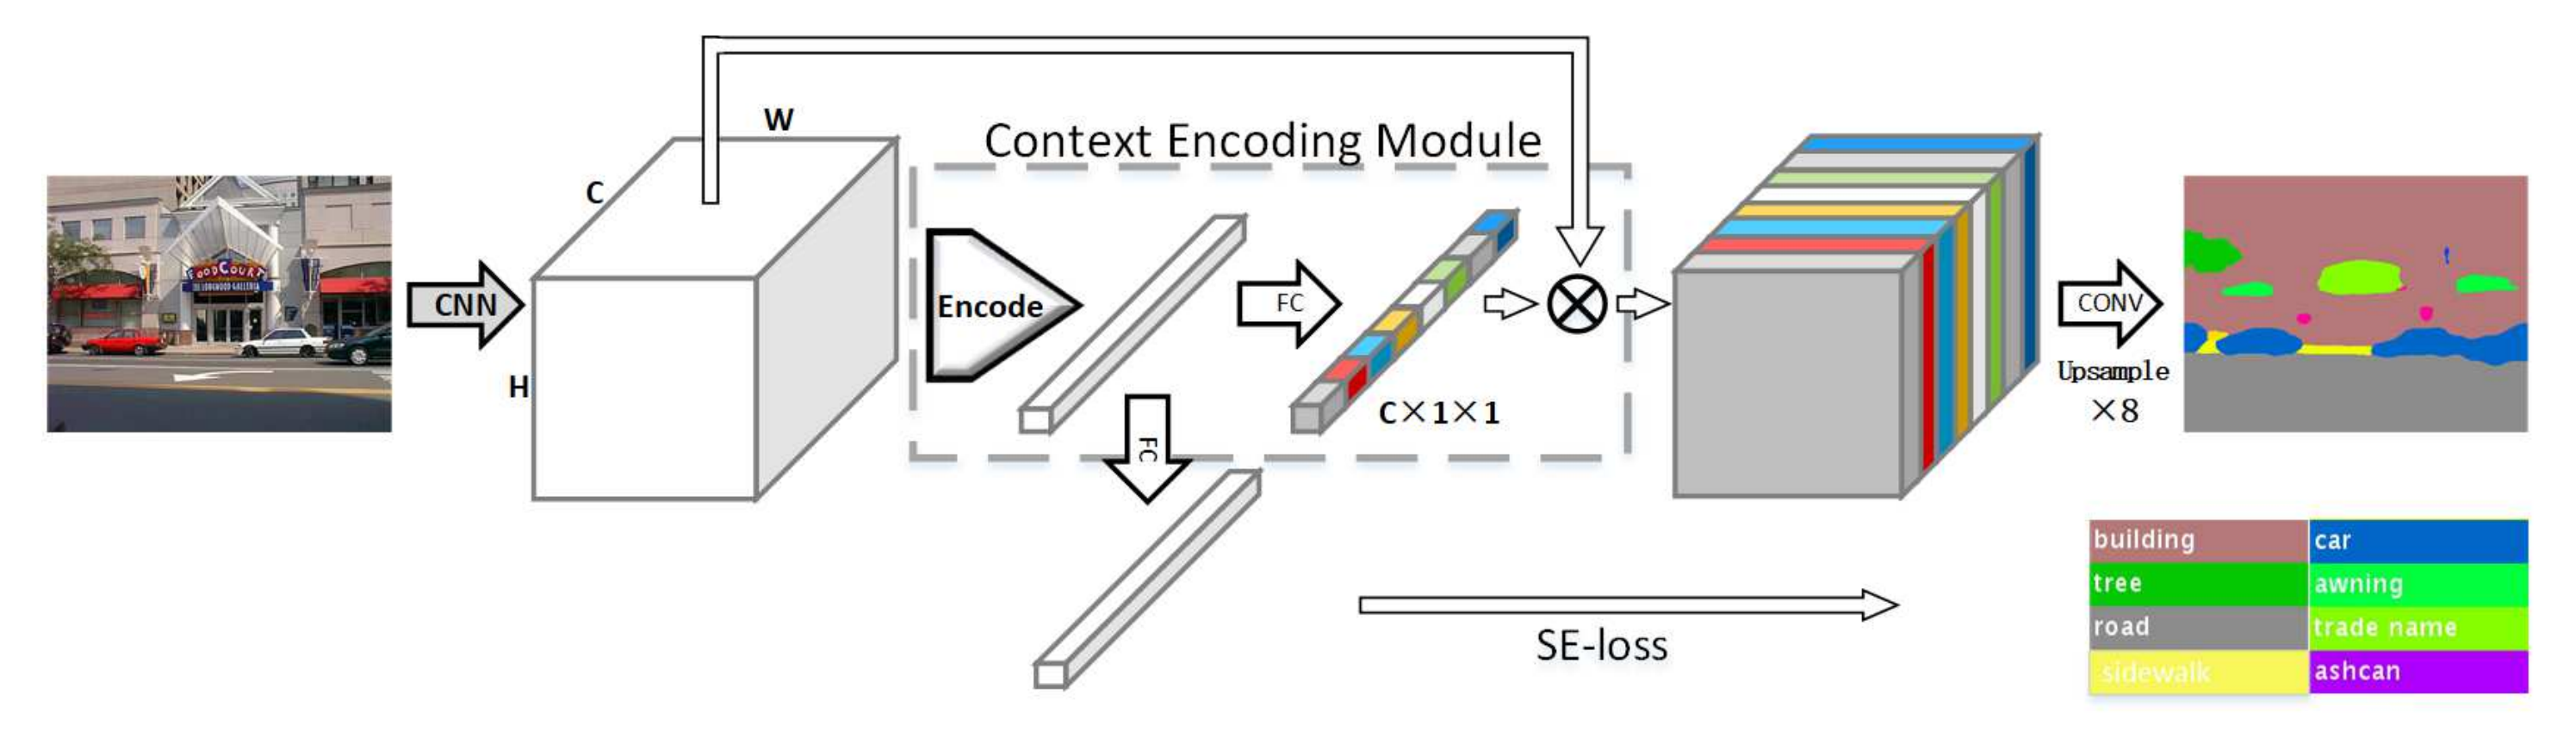
\includegraphics[width=\imgWidthXL]{images/context_encoding_module.png}
    \caption[Architecture based on \acf{CEM}]{Modified \ac{FCN} with \acf{CEM}: The class-dependent feature maps are shown within the \ac{CEM} prior to calculating the SE loss. The SE loss is employed to regularize the training of the \ac{CEM}, capturing a broader context than the standard per-pixel loss. Image from \cite{https://doi.org/10.48550/arxiv.1803.08904}.}
    \label{context_encoding_module}
\end{figure}

\squote{Shape-aware Instance Segmentation} \cite{DBLP:journals/corr/HayderHS16} from 2016 introduces a new approach to instance-level semantic segmentation, which is the task of jointly detecting, segmenting, and classifying individual objects in an image.\cite{hafiz2020survey}\cite{bolya2019yolact}. The presented methods use bounding boxes as candidate objects and directly predict a binary mask within each box. As this makes them sensitive to errors in the object proposal generation process, such as too small or shifted boxes, the authors propose a new object segment representation based on the distance transform of the object masks. This representation allows robust prediction of masks beyond the bounding boxes' scope. They subsequently design an \acf{OMN} to infer and decode this representation into the final binary object mask. The \ac{OMN} is integrated into a multi-task network cascade framework to learn the \acf{BAIS} network end-to-end. \figref{boundary_aware_instance_segmentation} contains further information about the architecture used. Experiments on the PASCAL VOC 2012 \cite{pascal-voc-2012} and CityScapes \cite{cordts2016cityscapes} datasets show the benefits of the proposed approach, outperforming the state-of-the-art in object proposal generation\footnote{Object proposal generation is a task in \ac{CV} that aims to generate candidate regions that are likely to contain objects of interest in images. It can be used as a preprocessing step for object recognition models to decrease the search space, improve efficiency and accuracy.\cite{https://doi.org/10.48550/arxiv.2201.06696}\cite{https://doi.org/10.48550/arxiv.2008.05700}\cite{objectProposalGeneration2021}} and instance segmentation.

\begin{figure}[H]%[htbp]
    \centering
    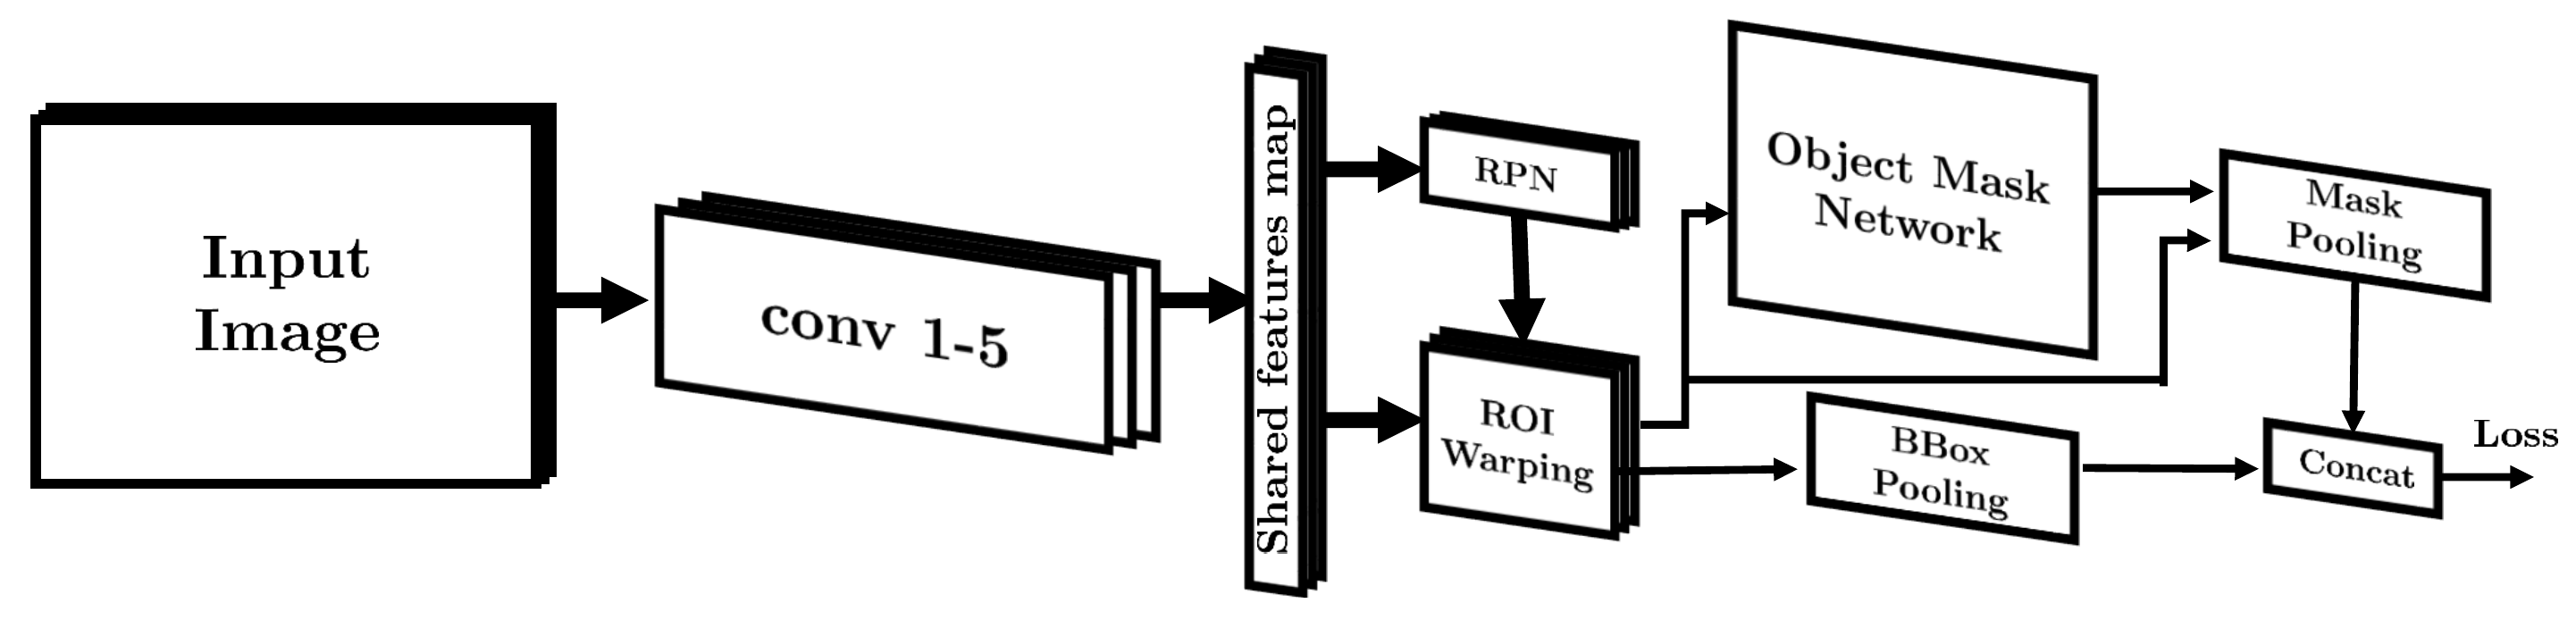
\includegraphics[width=\imgWidthXL]{images/boundary_aware_instance_segmentation.png}
    \caption[Shape-aware instance segmentation network]{The shape-aware instance segmentation network has an input image go through convolutional layers and a \ac{RPN}\cite{NIPS2015_14bfa6bb} for bounding box proposals, then \ac{RoI} warping and \ac{OMN} for binary mask generation, followed by feature extraction for classification. The 5-stage \acf{BAIS} network adds two more stages (OMN and classification module) to the initial three stages. The model uses a multi-task loss during training to encode errors in the bounding box, segmentation, and classification. Image from \cite{NIPS2015_14bfa6bb}.}
    \label{boundary_aware_instance_segmentation}
\end{figure}

\section{Multi-scale Processing}
Multi-scale processing is a technique to extract information from data at multiple scales. It involves processing the data at different resolutions or levels of detail to capture the complete structural information present in the data. The paper \squote{A Review on Multiscale-Deep-Learning Applications}\cite{Elizar2022-ey} from 2022 divides multi-scale \ac{DNN}approaches in two categories: multi-scale feature learning and multi-scale feature fusion where the former aims to extract feature maps by examining kernels over several sizes to collect a more extensive range of relevant features and the latter uses features with different resolutions to find patterns over short and long distances. These methods can be implemented as different architectures described in \figref{multi_scale_deep_learning}.

\squote{Multi-Scale Self-Guided Attention for Medical Image Segmentation} \cite{9066969} from 2021 presents a new approach to overcome the limitations of existing \ac{CNN} models related to redundant use of information and the lack of efficiently modeling long-range feature dependencies resulting in non-optimal discriminative feature representations\footnote{Non-optimal discriminative feature representations are feature representations that are not correctly suited for distinguishing different classes or categories\cite{chen2017discriminative}. They may contain noise or irrelevant information that reduces the accuracy or efficiency of pattern recognition \cite{Guo2020}.}. The paper describes a multi-scale guided attention network where four feature maps are extracted from 4 ResNet-101 at multiple scales and subsequently fed to a guided attention module with the benefit of removing noisy areas and helping the network emphasize the regions more relevant to semantic classes. \figref{multi_scale_self_guided_attention} further explains the concept of this approach. The model was evaluated on three datasets: abdominal organs, cardiovascular structures, and brain tumors. The results of the ablation experiments support the importance of the attention modules in the proposed architecture. The model outperformed state-of-the-art segmentation networks with improved accuracy and reduced standard deviation.

\begin{figure}[H]%[htbp]
    \centering
    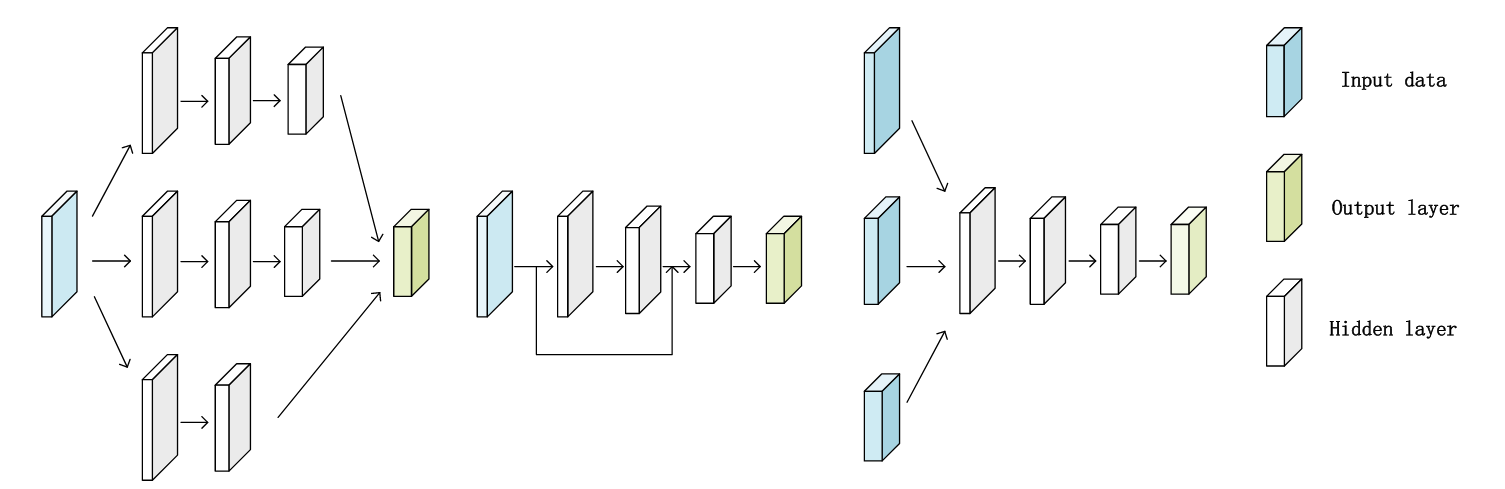
\includegraphics[width=\imgWidthXL]{images/multi_scale_deep_learning.png}
    \caption[Multi-scale processing architectures]{Summary of different multi-scale deep learning architectures described in \cite{10.1007/s10489-018-1150-1}. The left part shows a multi-column network where the input data is propagated into multiple parallel operating branches and concatenated as the final output. The middle part is the skip-net which merges low-level and high-level features as the output, whereas the right part is called multi-scale input, which resizes images to different scales before feeding them to the network. Image from \cite{10.1007/s10489-018-1150-1}.}
    \label{multi_scale_deep_learning}
\end{figure}

\begin{figure}[H]%[htbp]
    \centering
    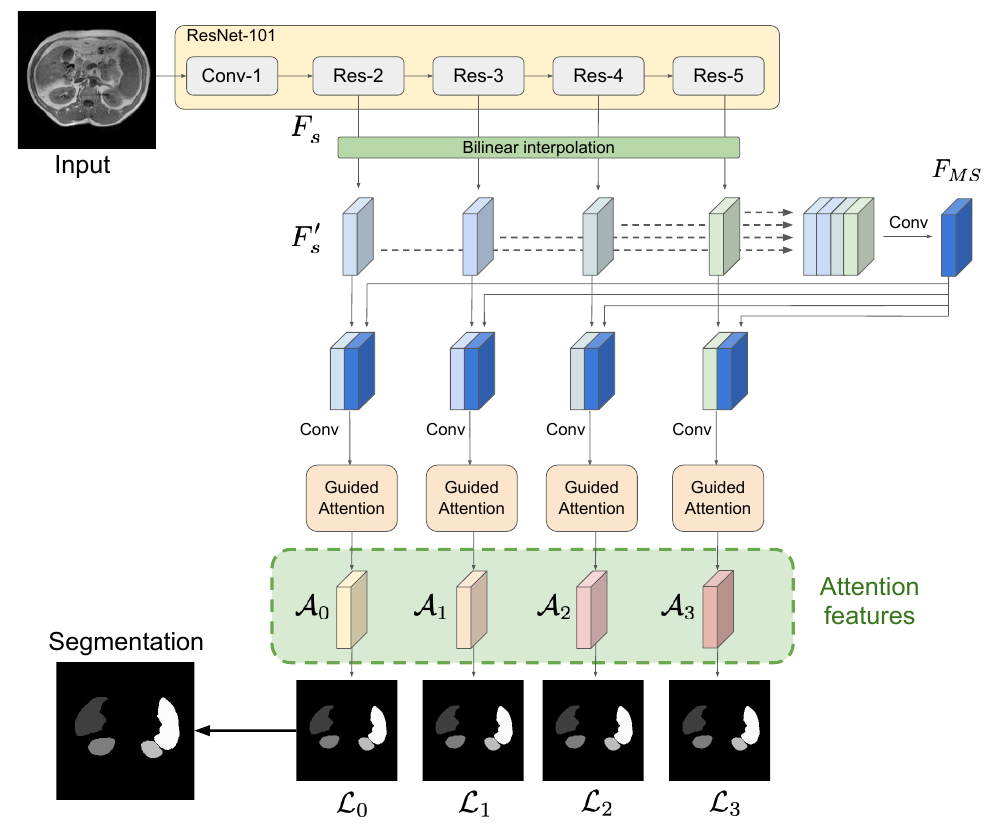
\includegraphics[width=\imgWidthXL]{images/multi_scale_self_guided_attention.png}
    \caption[Multi-scale attention network]{Architecture of the multi-scale guided attention network. Image from \cite{9066969}.}
    \label{multi_scale_self_guided_attention}
\end{figure}

\squote{Multi-Scale Context Aggregation for Semantic Segmentation of Remote Sensing Images} \cite{rs12040701} from 2020 presents a novel architecture for semantic segmentation of \acp{RSI} proposing a network called \ac{HRNet}. The \ac{HRNet} is designed to produce high-resolution features without the decoding stage and overcome the limitations of conventional encoder-decoder-based \acp{CNN}, which results in loss of localization accuracy and preservation of spatial details. The proposed architecture enhances the low-to-high features extracted from different branches to strengthen the embedding of scale-related contextual information. The low-resolution features are utilized to model long-term spatial correlations, while high-resolution branches are enhanced with an \ac{ASP} module to aggregate more local contexts. See \figref{multi_scale_context_aggregation} to view a schematic of the proposed model. The resulting architecture can exploit spatial context at both global and local levels\footnote{Local spatial context is related to information within a small region or neighborhood of the pixels, whereas global spatial context refers to the information across the whole image.}, achieving state-of-the-art performance on two \ac{RSI} datasets.

\begin{figure}[H]%[htbp]
    \centering
    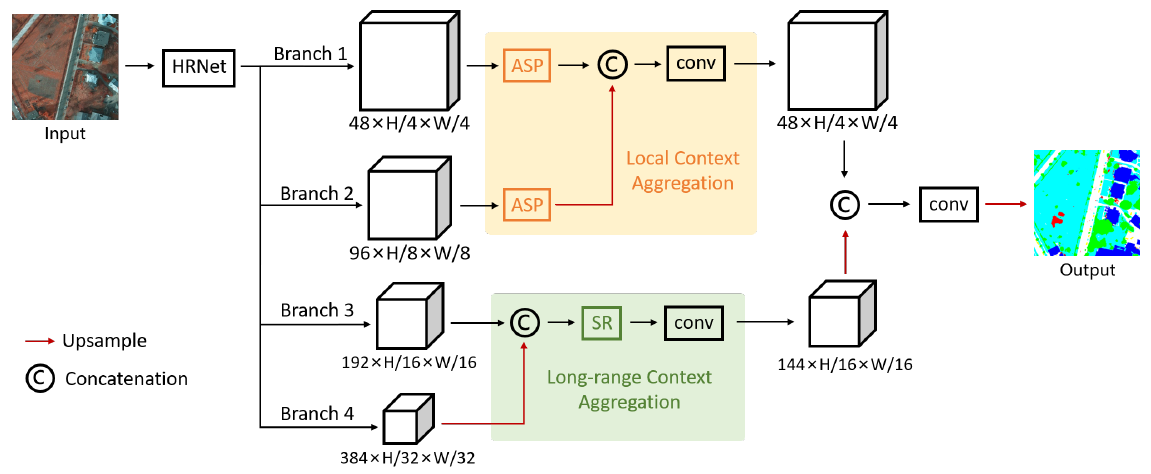
\includegraphics[width=\imgWidthXL]{images/multi_scale_context_aggregation.png}
    \caption[\acf{HRNet}]{\ac{HRNet} proposed by \cite{rs12040701}}
    \label{multi_scale_context_aggregation}
\end{figure}
\newpage

\section{Ensemble Learning}
The paper \squote{A survey on ensemble learning} \cite{Dong2020} presents an excellent review of the field of ensemble learning, a machine learning technique that combines multiple models to make predictions. The paper begins by introducing the concept of ensemble learning and its history, tracing its roots back to the 1960s and 1970s. The author then categorizes ensemble methods, including bagging, boosting, stacking, and hybrid.

\begin{wrapfigure}{r}{0.4\textwidth}
    \centering
    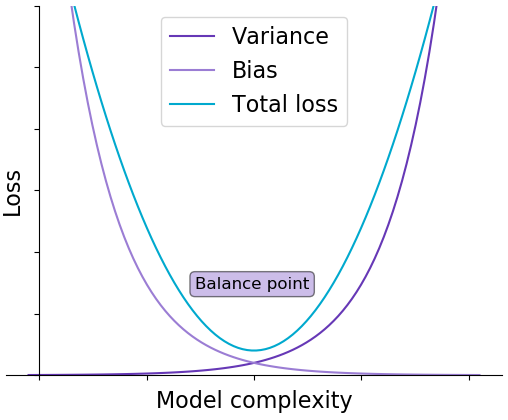
\includegraphics[width=0.30\textwidth]{images/relationship_learningcurve_complexity.png}
    \captionsetup{width=0.30\textwidth}
    \caption[Learning curve and model complexity]{Relationship between complexity and learning curve \cite{Dong2020}}
    \label{relationship_learningcurve_complexity}
    \vspace{-20pt}
\end{wrapfigure}

Bagging, or bootstrap aggregating, is a technique that trains multiple models on different subsets of the training data generated using bootstrapping and combines the predictions of these models to make a final prediction. Conversely, Boosting trains models sequentially, giving more weight to samples than previous models in the sequence misclassified. Stacking involves training a meta-model on the predictions of multiple base models, and hybrid methods are combinations of bagging and boosting.

The impact of those techniques on the relationship between the learning curve and model complexity can be summarized as follows:

\textbf{\emph{Bagging}} reduces variance and can lead to smoother learning curves as the models are trained on different subsets of the data. The model complexity remains the same.

\textbf{\emph{Boosting}} reduces bias and can lead to a faster decrease in training error in the beginning, but it can also lead to overfitting if the model complexity is too high. The model complexity increases with each iteration as the model focuses on the samples that were misclassified.

\textbf{\emph{Stacking}} combines the predictions of multiple models, leading to a reduction in variance, and can improve the model's overall performance.

\textbf{\emph{Hybrid Methods}} affect the relationship between the learning curve and model complexity depending on the specific combination of bagging and boosting. However, the overall effect is reduced variance and bias, which can result in smoother and faster convergence of the learning curve.

The assessment and comparison of ensemble methods are also covered in the study, along with several techniques for choosing the optimal ensemble and performance indicators like accuracy and F1-score. The author also emphasizes the difficulties and restrictions of ensemble learning, such as the danger of overfitting and the difficulty in choosing suitable base models.

The paper's discussion outlines the importance of ensemble learning for numerous applications in fields such as computer vision, natural language processing, and bioinformatics.

\squote{A Systematic Evaluation of Ensemble Learning Methods for
{Fine-Grained} Semantic Segmentation of {Tuberculosis-Consistent}
Lesions in Chest Radiographs} \cite{Rajaraman2022-fy} from 2022 evaluates the performance of different ensemble learning methods for fine-grained semantic segmentation of tuberculosis-consistent lesions in chest radiographs. The study compares the performance of several ensemble methods, including bagging, boosting, and stacking, on a dataset of chest radiographs. The study results show that the stacking method performed better than the other ensemble methods, providing improved performance over the individual models regarding accuracy and computation time. The paper concludes that stacking is a promising approach for fine-grained semantic segmentation in chest radiographs and highlights the importance of considering different ensemble methods for such tasks. \figref{ensemble_tuberculosis} describes the setup for this method.

\begin{figure}[H]%[htbp]
    \centering
    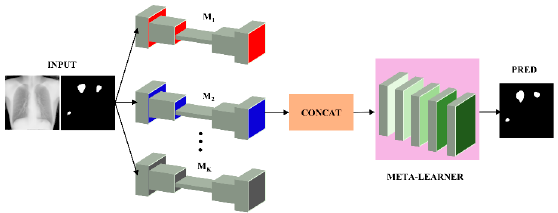
\includegraphics[width=\imgWidthXL]{images/ensemble_tuberculosis.png}
    \caption[Stacking ensemble]{Stacking ensemble using the top-K models $M_1,M_2,\cdots M_k$ as input for a fully-convolutional meta-learner. After the top-K models are initialized with their trained weights, the features from the penultimate layers are extracted and concatenated. Subsequently, the meta learner is used for second-level learning \protect\footnotemark. Image from \cite{Rajaraman2022-fy}.}
    \label{ensemble_tuberculosis}
\end{figure}
\footnotetext{Second-level learning is a machine learning technique that involves training a model to learn how to select predictions of other models.\cite{Breiman1996}\cite{WOLPERT1992241}}

\squote{Ensemble Knowledge Transfer for Semantic Segmentation} \cite{8354272} from 2018 presents a method for transferring knowledge from existing datasets to a new target dataset for aerial semantic segmentation. The authors introduce AeroScapes, a new dataset of 3269 aerial images annotated with semantic segmentation. To transfer knowledge, the authors use transfer learning techniques to train multiple models for aerial segmentation by fine-tuning through each source domain. See \figref{ensemble_knowledge_transfer}. The models are then combined into an ensemble. This results in significant improvements (8.12\%) in performance over standard baselines.
\begin{figure}[H]%[htbp]
    \centering
    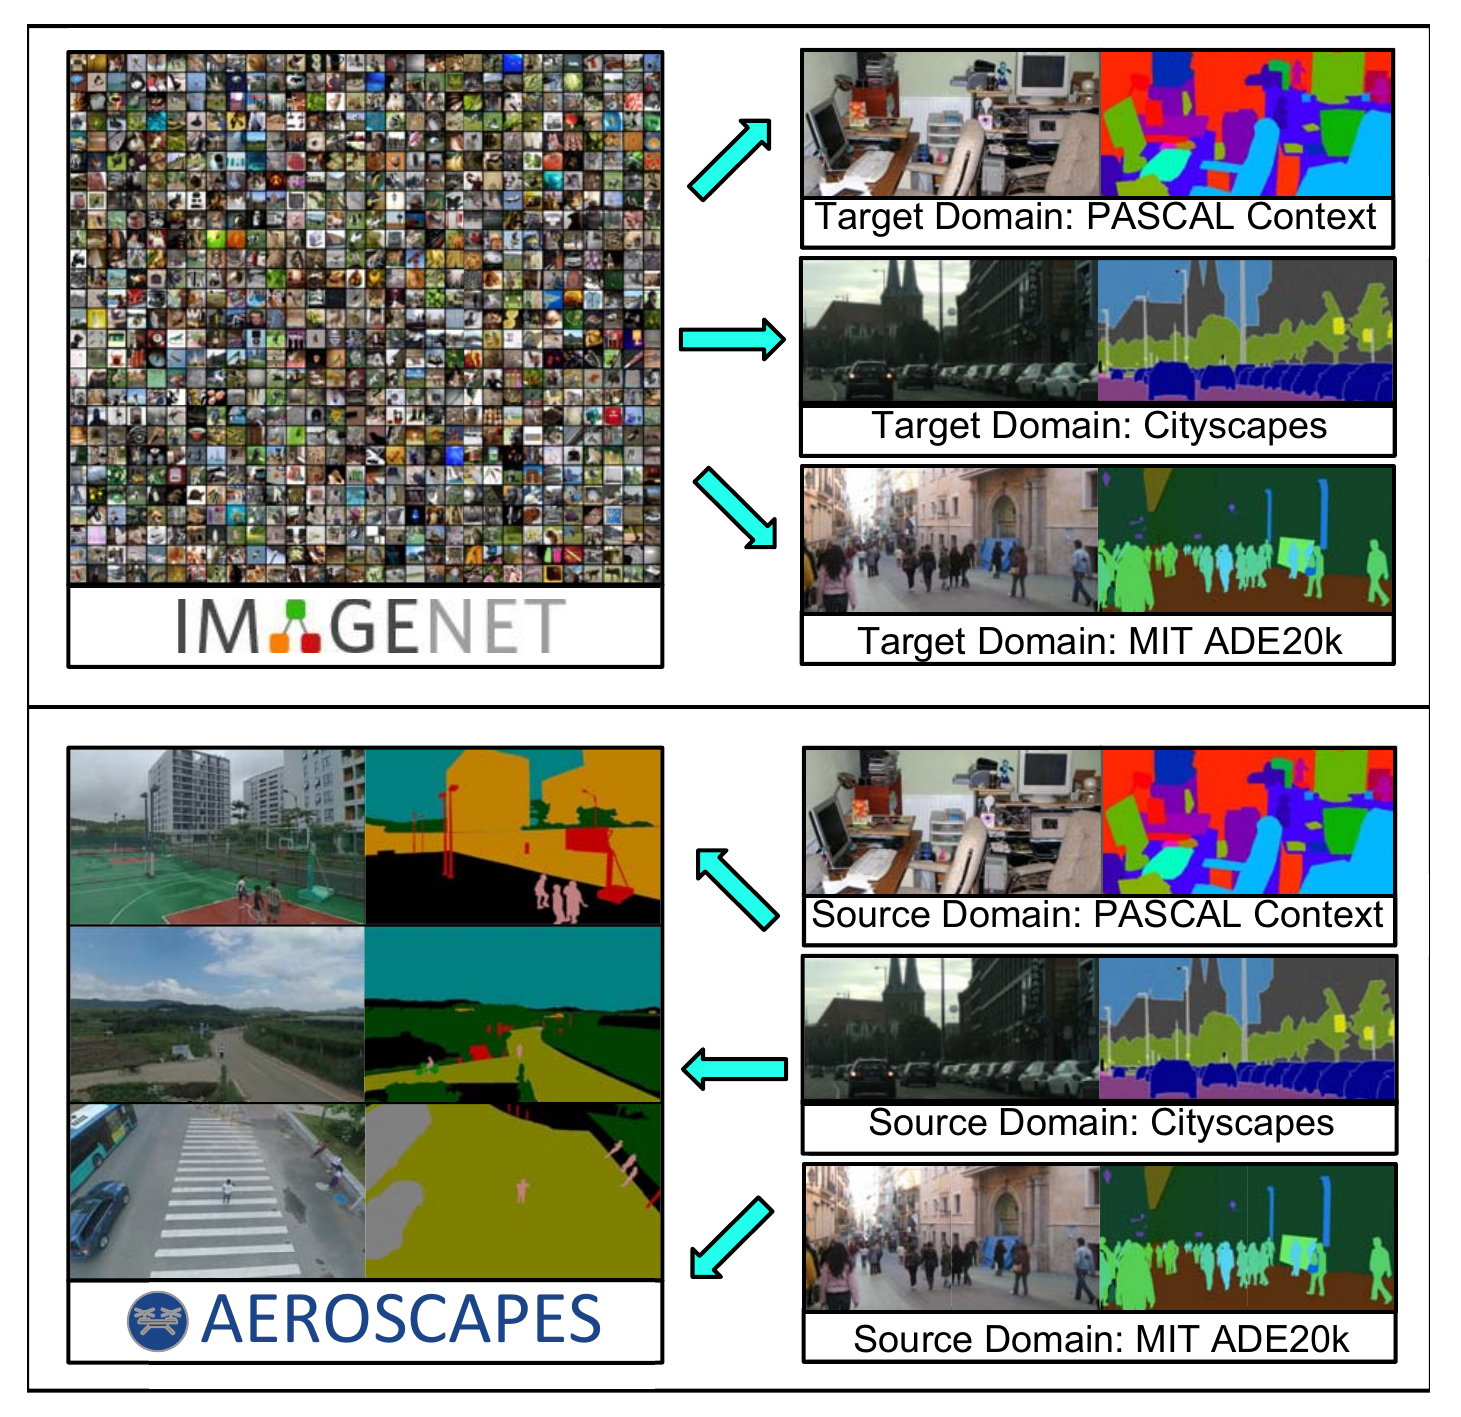
\includegraphics[width=\imgWidthXL]{images/ensemble_knowledge_transfer.png}
    \caption[Multi-target and single-target knowledge]{Instead of taking advantage of multi-target knowledge transfer (top row), the paper introduces a new technique where specific source domains are fine-tuned to make predictions to a single target domain (bottom row). The concept is called multi-source knowledge transfer. Image from \cite{8354272}.}
    \label{ensemble_knowledge_transfer}
\end{figure}

\section{Transfer Learning}
The paper \squote{A Comprehensive Survey on Transfer Learning} \cite{DBLP:journals/corr/abs-1911-02685} from 2019 provides an excellent survey on transfer learning. The authors define transfer learning as improving the performance of target learning on target domains by transferring the knowledge contained in different but related source domains. Note that the two domains should be somehow related to each other. For example, if we train a model to recognize images of cats, we can reuse that model to recognize images of dogs. Even if cats and dogs are not within the same domain, they are related in terms of being both mammals with four legs and fur and generally with similar features. If the source domain is entirely different from the target domain, successfully reusing a model may be more challenging.
An example could be a model trained to recognize text sentiment in English and then reused to recognize text sentiment in a different language. The features might be completely different, making the transfer of knowledge much more challenging. The following section will provide more information on transfer learning related to increased semantic segmentation performance.

\squote{Transfer Learning via Parameter Regularization for Medical Image Segmentation} \cite{9616331} from 2021 presents a new method which aims to reduce \squote{catastrophic forgetting} \cite{mccloskey1989catastrophic} which is a tendency of a network to forget previously learned information when learning new information thoroughly. The authors state that target models are not expected to handle the source task and therefore need to remember it. They propose a transfer learning method that addresses this \squote{forgetting problem} by using the parameters of the source network as a regularization instead of an initialization term. The learned parameters of the target model are penalized if they deviate too far from the source network, which helps to overcome the catastrophic forgetting problem and take advantage of the knowledge obtained by the source model. This transfer learning strategy is applied to COVID-19 opacity segmentation and improves the segmentation of coronavirus lesions in chest CT scans.

\squote{Distant Domain Transfer Learning for Medical Imaging} \cite{9325521} from 2021 presents a transfer learning method that obtains knowledge from multiple unlabeled source domains to improve accuracy for training on a labeled target domain to classify CT scans of COVID-19 patients. The source domains do not have to be related to the target domain as in common transfer learning methods. The method is inspired by the fact that even if domains seem unrelated on the instance level, there might still be common properties on the feature level. The authors propose a three-staged process defined as
\begin{equation}
    \mathop{\min}_{\theta_E,\theta_D \Theta_C} L = L_R + L_D + L_C
    \label{eqn:distant_domain_transfer_loss}
\end{equation}
where $L_R$ consists of a reconstruction loss obtained from an autoencoder with multiple sources and one target domain. The goal is to create robust, unsupervised features that are then forwarded to obtain $L_D$, which is the domain loss responsible for closing the distance between the source and target domains, necessary to avoid the distribution mismatch between the source and target domains and provide robust, domain-invariant\footnote{Domain-invariant features are features that remain consistent across different domains or datasets. In machine learning, a \textit{domain} is defined as a specific distribution of data, such as images of humans versus images of animals.} features. The method used in this step is called \squote{maximum mean discrepancy} \cite{turchenko2017deep}. The last part of \ref{eqn:distant_domain_transfer_loss} is the classification loss $L_C$, which is obtained by a fully connected layer added to the encoder of the network. The loss takes samples and output labels from the target domain and complements them as the final component to the overall objective $L$. Even if the results achieve excellent performance in COVID-19 and pneumonia diagnosis, the method has some drawbacks: case-specificity, complicated source domain selection, and computationally expensive calculation of $L_D$.

\section{Weakly-supervised Learning}
As mentioned in \secref{subsec:unsupervised_learning}, weakly-supervised learning only uses partial information about the label. The paper \squote{A brief introduction to weakly supervised learning} \cite{10.1093/nsr/nwx106} from 2017 provides a detailed introduction of weakly supervised learning and further specifies weakly supervised learning in \squote{incomplete supervision} which only uses a subset of training data and labels, \squote{inexact supervision} where labels are coarse-grained\footnote{Coarse-grained labels are also called high-level labels which are used to categorize data in a very general and simplified way. Instead of specifying the type of animals in images, coarse-grained labels could provide \squote{animal} as the labeled category.}, and \squote{inaccurate supervision} where the given labels are not always ground-truth labels. The following reviews will cover weakly-supervised techniques related to semantic segmentation.

\squote{Going to Extremes: Weakly Supervised Medical Image Segmentation} \cite{make3020026} from 2021 proposes a new method for segmenting medical images. The techniques aim to reduce the general effort of generating new training datasets by minimizing manual intervention to just a few clicks. The method consists of three steps. The first step is to create an initial segmentation based on the extreme points annotated manually. The points identify the regions of interest and are subsequently provided as input to the \squote{random walker algorithm}. The algorithm can be used for simple segmentation using a set of known labeled pixels to determine the labels of other pixels \cite{grady2006random}. The initial segmentation is then used as \squote{noisy supervision} to train a \ac{CNN} to segment organs of interest. The authors claim this type of initialization is relatively robust for six different tasks from medical image segmentation. The third step consists of fine-tuning the network through multiple training iterations. The results show that the proposed model generalizes to unseen data with limitations for organs with diverse interior textures or extremely concave curved shapes, such as the pancreas.

\squote{Learning Pixel-Level Semantic Affinity With Image-Level Supervision for Weakly Supervised Semantic Segmentation} \cite{Ahn_2018_CVPR} from 2018 present a \ac{DNN} called AffinityNet that predicts semantic affinities on pixel-level while originally trained with image-level class labels only. Image-level labels only indicate the existence of a particular object class and do not inform about object location or shape, which are essential for semantic segmentation. The authors employ the \ac{CAM} technique \cite{zhou2016learning} to achieve a rough localization. \ac{CAM} is a method used to generate visualizations of the significant regions in an image that contribute to a feasible classification decision because the proposed AffinityNet was trained using image-level class labels. As illustrated in \figref{weakly_affinity}, affinity labels are derived from the \ac{CAM} by sampling pairs of neighboring coordinates and assigning labels based on class consistency. Affinity labels and training images are then used to train AffinityNet, which outputs semantic affinities within local image areas\footnote{In computer vision, local image areas refer to specific regions or patches of an image that are smaller in size than the entire image. These local areas can be used for various tasks, such as object detection, image segmentation, and feature extraction.}. With the \ac{CAM}, those predictions are then used with the random walk algorithm \cite{grady2006random} to create output labels for a semantic segmentation network. The authors claim to achieve state-of-the-art performance for models trained with equal supervision and even outperform some older supervised models from the \squote{early days}\cite{long2015fully}.

\begin{figure}[H]%[htbp]
    \centering
    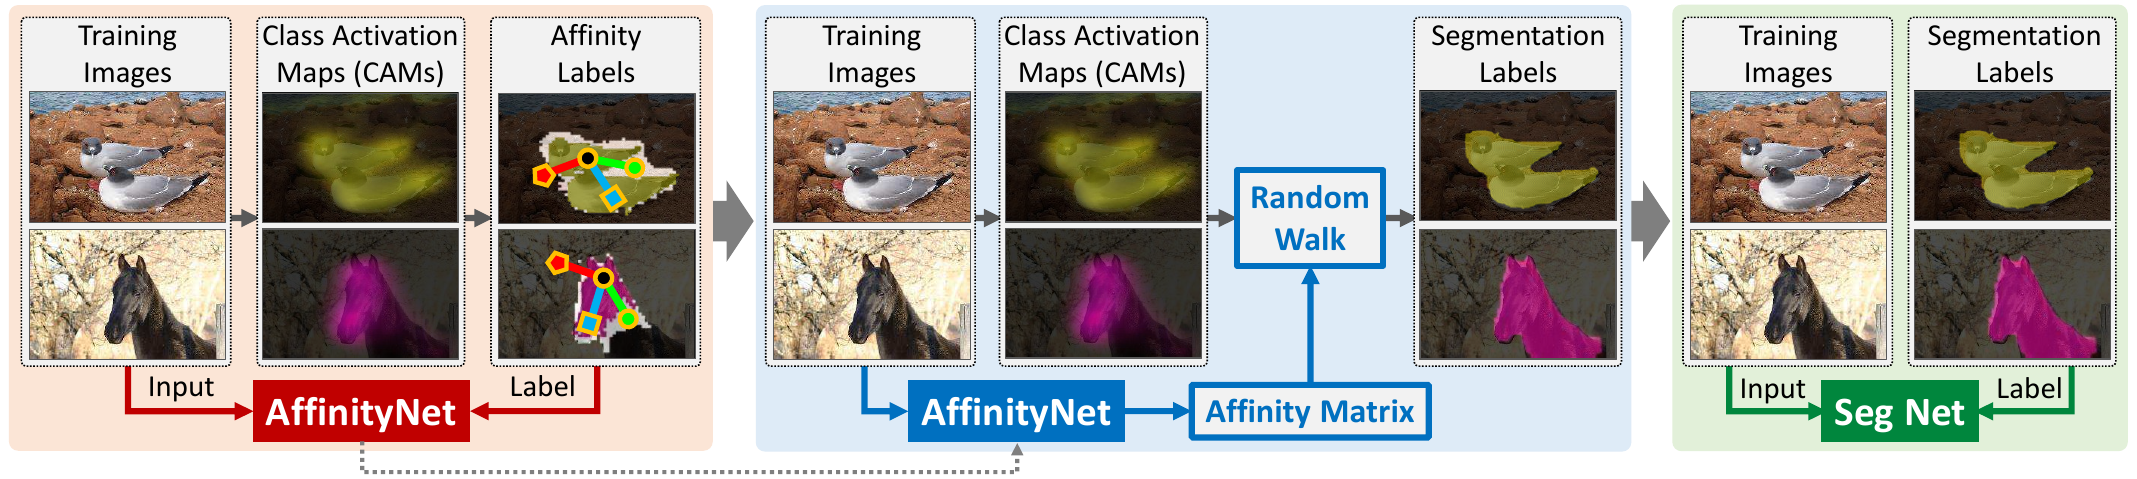
\includegraphics[width=\imgWidthXL]{images/weakly_affinity.png}
    \caption[AffinityNet]{Visual concept of AffinityNet and SegNet. The image is taken from \cite{Ahn_2018_CVPR}}
    \label{weakly_affinity}
\end{figure}

\section{Active Learning}
\ac{AL} is a \ac{ML} method where the algorithm chooses the most informative data points from an unlabeled dataset and asks the user to label them, which helps to reduce the number of labeled data necessary for training \cite{settles2009active}. See \figref{active_learning_cycle} for further information. There are several approaches to selecting informative data, such as uncertainty-based sampling \cite{sharma2017evidence} or diversity-based \cite{4036653} sampling. Uncertainty-based sampling is an active learning strategy that selects data points that are the most uncertain and, thus, are highly informative. Uncertainty in this context refers to what degree of confidence the model has in its predictions for certain data points. Examples of uncertainty-based sampling are query-by-committee \cite{kee2018query} and maximum entropy sampling \cite{mayer2020adversarial}. Diversity-based sampling aims to select data points that are diverse or different from those labeled already. Here the goal is to capture the full diversity of the data, which can be useful where labeled data is biased towards a particular subset \cite{agarwal2020contextual}. Some examples include density-weighted active learning \cite{donmez2007dual} or uncertainty sampling with diversity \cite{wang2017uncertainty}.

\begin{figure}[H]%[htbp]
    \centering
    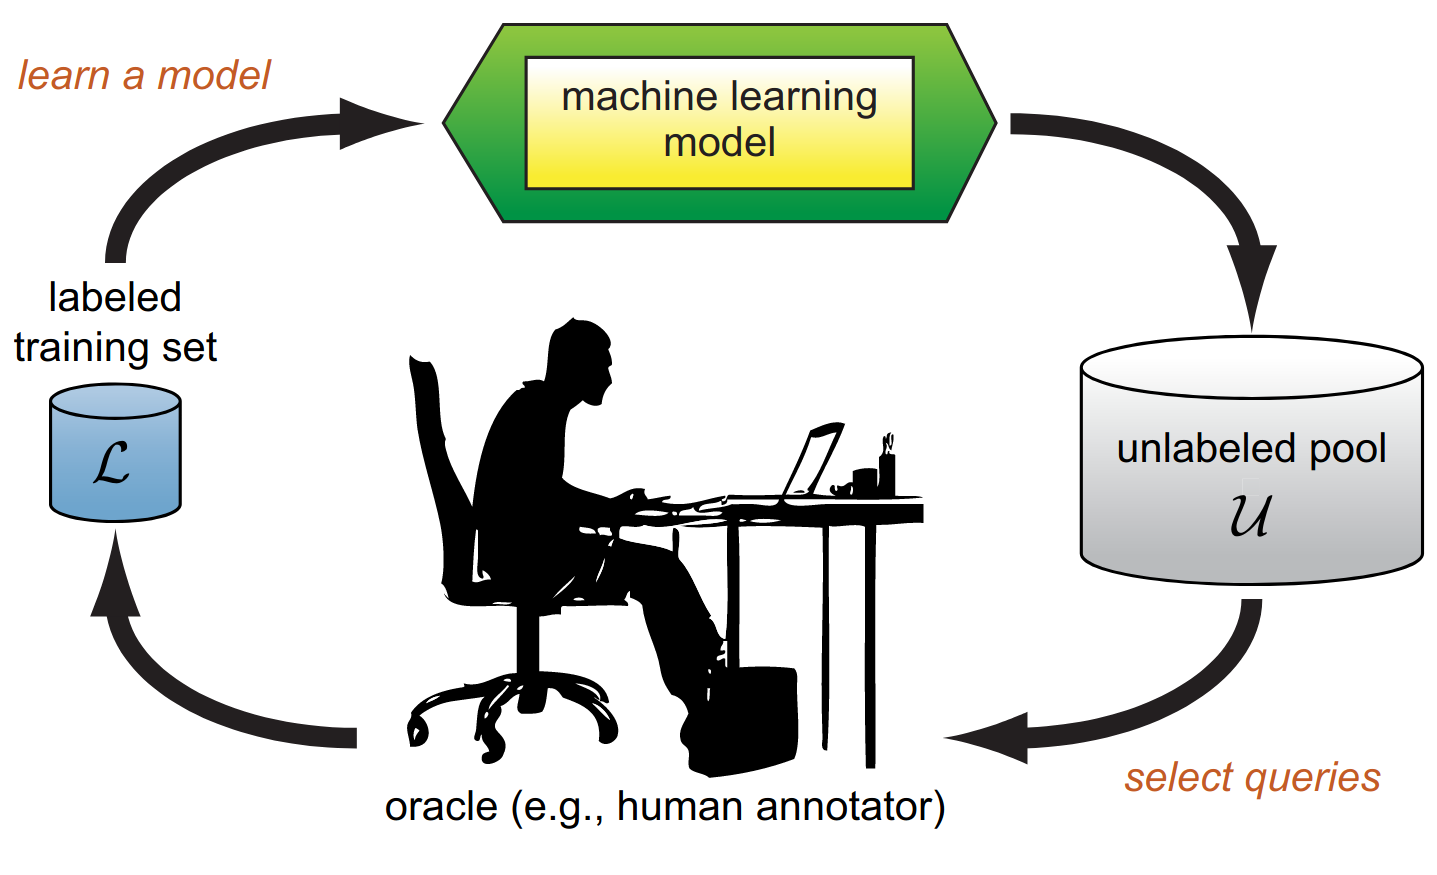
\includegraphics[width=\imgWidthM]{images/active_learning_cycle.png}
    \caption[\acf{AL} cycle]{\acf{AL} cycle. Image from \cite{settles2009active}}
    \label{active_learning_cycle}
\end{figure}

\squote{A Survey on Active Learning and Human-in-the-Loop Deep Learning for
Medical Image Analysis} \cite{DBLP:journals/corr/abs-1910-02923} from 2019 presents an extensive survey of active learning and human-in-the-loop deep learning methods for medical image analysis. The authors discuss the importance of \ac{AL} techniques by addressing the challenges of small data sets, high annotation costs, and large inter- and intraobserver variability\footnote{Interobserver variability is the variation in annotations made by different annotators when analyzing the same medical image. This variability can occur due to different training, expertise, or perception pieces. Intraobserver variability is the variation in annotations made by the same annotator caused by fatigue or lack of standardized annotation procedures.\cite{hopper1996analysis}} when annotating medical data. The paper subsequently describes the active learning process, numerous strategies for selecting informative data points, and advantages such as better and faster results, less needed expertise for labeling tasks, and freeing up expert time.

\squote{ViewAL: Active Learning With Viewpoint Entropy for Semantic Segmentation} \cite{Siddiqui_2020_CVPR} from 2020 proposes a new active learning framework called ViewAL for semantic segmentation of 3D point clouds. The active learning strategy exploits inconsistent predictions across different image views, whereas traditional uncertainty sampling techniques operate on single images. The authors claim that single image sampling ignores geometric constraints\footnote{Geometric constraints refer to a set of rules or relationships between objects in space that describe how they are positioned, oriented, or related to each other. For further information on geometric constraints, see \cite{grimson1991object}.} which are essential when examining the quality of network predictions. Generally, the ViewAL framework involves four steps. The first step trains a regular model on a labeled dataset. The second step uses the trained model to predict unlabeled parts of the data. The third step selects superpixels with high uncertainty from the predictions, which are subsequently requested in the fourth step from a human annotator. The authors evaluate their framework on three public datasets called SceneNet-RGBD \cite{McCormac:etal:ICCV2017}, ScanNet\cite{dai2017scannet} and Matterport3D\cite{Matterport3D} achieving promising results.

\section{Semi-supervised Learning}
As defined in \secref{subsec:unsupervised_learning}, semi-supervised learning generally uses labeled and unlabeled data. The paper \squote{A survey on semi-supervised learning} from 2019 provides a relatively new survey of semi-supervised learning. The authors define semi-supervised learning as a branch that combines supervised and unsupervised learning to improve performance in one of these tasks by utilizing information associated with the other task. The article starts by covering basic concepts of semi-supervised learning methods and connecting the task to clustering. They further cover wrapper methods which include self-training, co-training, and boosting. After describing unsupervised processing, different intrinsically semi-supervised methods are covered, which aim to include unlabelled samples in the object function without relying on intermediate steps or supervised base learners. The article additionally covers transductive methods, which do not have a training and testing phase, unlike the previously mentioned methods. The significant difference between transductive methods is that they can only predict part of the input space. The predictions are restricted to the unlabelled set given in advance. The last section outlines future perspectives for semi-supervised learning to be a vital tool in uncovering complex structures in data. The authors also estimate that the distinction between clustering and classification will fade.

\squote{Casting Geometric Constraints in Semantic Segmentation as Semi-Supervised Learning} \cite{https://doi.org/10.48550/arxiv.1904.12534} from 2019 discusses the challenges of generalizing semantic segmentation to new indoor scenes even if trained with a large dataset such as SUNRGB-D \cite{song2015sun}. The problem is known as dataset bias, domain shift, sample selection bias, or class imbalance and root in the complexity of the visual world where datasets describe just some of its aspects \cite{tommasi2017deeper}. The authors of \cite{https://doi.org/10.48550/arxiv.1904.12534} propose to exploit geometric constraints as a semi-supervised term to create a model which can be used to segment target sequences of ScanNet\cite{dai2017scannet} using only annotations from SUNRGB-D. The proposed method is shown to be effective through quantitative and qualitative experiments.

\squote{Shape-aware Semi-supervised 3D Semantic Segmentation for Medical Images} \cite{DBLP:journals/corr/abs-2007-10732} from 2020 propose a novel shape-aware semi-supervised segmentation strategy. The authors develop a multi-task network that simultaneously predicts segmentation masks and signed distance maps. The signed distance maps are predicted for labeled and unlabelled data and combined within a proposed adversarial loss which is further combined with the regular segmentation loss. See \figref{shape_aware_semi_supervised_method} for further information on the exact layout, which allows the model to generalize to the unlabelled portion of the dataset by enforcing similar distance map distributions. Experiments show that the method outperforms current state-of-the-art approaches with improved shape estimation validating its efficacy.

\begin{figure}[H]%[htbp]
    \centering
    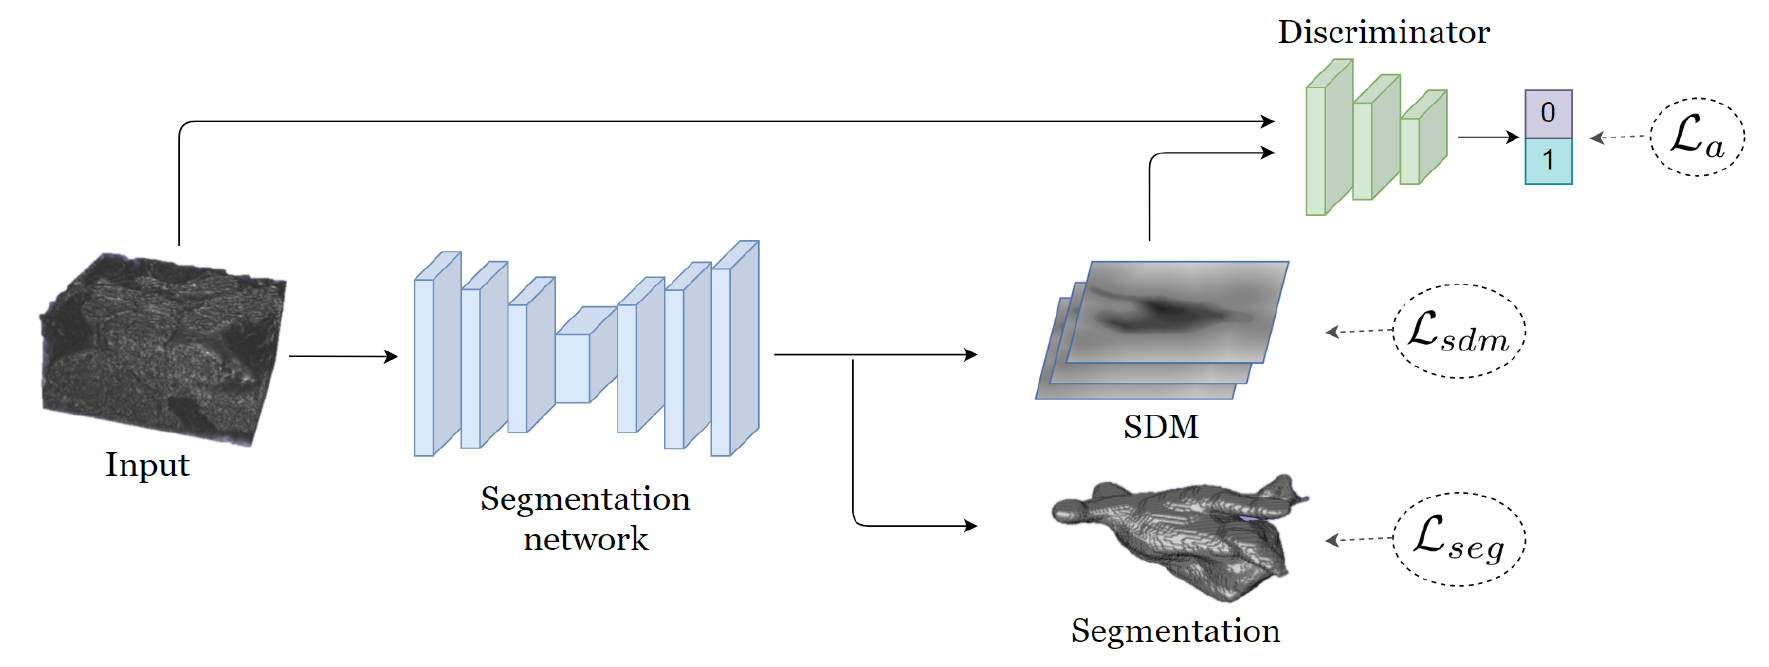
\includegraphics[width=\imgWidthXL]{images/shape_aware_semi_supervised_method.png}
    \caption[Shape aware semantic segmentation]{Framework of a semi-supervised shape aware implementation. The adversarial loss $\mathcal{L_{\alpha}}$ takes as input predictions from the labeled and unlabelled part of the dataset and serves as a regularization term to the model. Image from \cite{DBLP:journals/corr/abs-2007-10732}.}
    \label{shape_aware_semi_supervised_method}
\end{figure}

\section{Domain Adaption}
The paper \squote{Deep visual domain adaptation: A survey} \cite{Wang_2018} from 2018 provides a detailed summary about \ac{DA}. The authors define \ac{DA} as a case of transfer learning that utilizes labeled data in a source domain to execute new tasks in a target domain. There can be several differences when speaking about source and target domains. A significant difference is the distributional difference. The authors describe several factors, such as illumination, pose, or image quality which can cause differences between a source and a target domain. Another term for these differences is domain shift. An example of domain adaption would be to use a model trained with images from animals recorded in a zoo for images of animals recorded in the wild. \ac{DA} techniques attempt to solve these types of challenges. While numerous techniques exist for shallow \ac{DA}, the paper focuses on deep \ac{DA}. The difference is that the latter is a specific type of \ac{DA} focused on deep learning models. When describing the algorithms for \ac{DA}, the authors divide them into two categories called instance-based \ac{DA} and feature-based \ac{DA}.
To adapt a source domain to a target domain with \squote{instance-based methods}, one would have to train a model with specific weights for instances which would reduce the discrepancy between the source and target domain. In other words, we would first compute a weight for each instance in the source domain based on its similarity to the instance in the target domain and then use these weights to train a machine-learning model on the source domain. Instances with higher weights are given more importance during training, while instances with a lower weight are given less importance. To adapt a source domain to a target domain with \squote{feature-based methods}, we could identify the most relevant features for the target domain with techniques such as mutual information \cite{vergara2014review} or correlation analysis \cite{hardoon2004canonical}. The goal is to match the distribution of the target domain. Subsequently, we can increase or lower the weights to features depending on their relevance and train the model with the chosen weights. The model will then be more sensitive to the features most relevant to the target domain and less sensitive to the less relevant features. The following paragraphs present implementations of \ac{DA} within the context of semantic segmentation.

\squote{A Novel Domain Adaptation Framework for Medical Image Segmentation} \cite{DBLP:journals/corr/abs-1810-05732} from 2018 proposes a novel \ac{DA} strategy to face the scarcity of training data in medical imaging. The core idea is to create a synthetic dataset of tumor-bearing \ac{MR} images and adapt those to the domain of real images from BRATS \cite{Menze2014-gj}. The synthetic dataset is created with a custom process based on a partial differential equation tumor model \cite{subramanian2019simulation}, which captures the time evolution of enhancing and necrotic tumor concentrations of tumor-induced brain edema. As this synthetic dataset and the dataset from BRATS display a high difference in intensity distributions, a new model called \squote{CycleGAN} is introduced to perform domain adaption from the synthetic to the real dataset. \squote{CycleGAN} is defined as
\begin{equation}
    G:X \to Y
\end{equation}
where $X$ is the synthetic data and $Y$ the real data. The goal is to learn the mapping $G$ such that the distribution of images from $G(X)$ are indistinguishable from the distribution of $Y$ by using an adversarial loss \footnote{An adversarial loss is a loss function used in \acf{GAN}\cite{https://doi.org/10.48550/arxiv.1511.05644}, a type of \ac{NN} architecture used for generating realistic data, such as images \cite{yi2019generative}, audio \cite{donahue2018adversarial}, or videos \cite{yu2022generating}.} The \ac{DA} approach is then combined with a custom segmentation method achieving promising results on the BRATS 18 data. They further claim to have augmented the existing data by twice the number of brain images.

\squote{Synergistic Image and Feature Adaptation: Towards Cross-Modality Domain Adaptation for Medical Image Segmentation} \cite{Chen_Dou_Chen_Qin_Heng_2019} from 2019 proposes a new unsupervised domain adaption framework called \ac{SIFA}. Their framework aims to address the problem of domain shift in deep learning. The authors describe their approach as a combination of feature and image adaptions to transform domain-invariant\footnote{Domain invariance refers to the ability of a model or algorithm to perform well on data from a domain that is different from the one on which it was trained. In other words, a model or algorithm that exhibits domain invariance can generalize its performance to new, unseen data from different domains. For further information, see \cite{tzeng2014deep}.} features and image appearance for a segmentation task in a target domain. Feature and image adaptions refer to the concept of feature and instance-based methods described above. \ac{SIFA} is validated on cross-modality medical image segmentation of cardiac structures, which refers to segmenting different anatomical structures through different imaging modalities such as magnetic resonance or computed tomography. The results show that \ac{SIFA} recovers performance degradation caused by domain shift and outperforms state-of-the-art methods after applying their \ac{DA} technique.

\section{Post-processing}
Post-processing for semantic segmentation refers to a set of techniques applied to the output of a segmentation algorithm to increase their quality and accuracy. Some standard post-processing techniques used in semantic segmentation are noise reduction \cite{van2003noise}, edge detection \cite{shrivakshan2012comparison}, morphological operations \cite{chudasama2015image}, conditional random fields \cite{8991232}, region merging or region splitting \cite{patil2013medical}. The following paragraphs summarize some specific post-processing methods for segmentation.

\squote{Anatomical Priors for Image Segmentation via Post-Processing with Denoising Autoencoders} \cite{https://doi.org/10.48550/arxiv.1906.02343} from 2019 introduces a new technique called Post-DAE which stands for post-processing with denoising autoencoders. The idea is to produce anatomically plausible segmentations by improving pixel-level predictions in a post-processing fashion from any classifier. 
    The denoising autoencoder is defined as
\begin{equation}
    \mathcal{L}_{DAE}(S_i)=DSC(S_i,f_{dec}(f_{enc}(\phi(S_i))))
\end{equation}
where $S_i$ is an anatomically plausible segmentation mask that is attempted to be reconstructed after being transferred in a lower dimensional space. The function $\phi(S_i)$ is part of a mask degradation strategy and aims to produce noisy segmentations used for training. The authors suggest the \ac{DL} as a loss function as an objective to minimize. Once the model is trained, any prediction from any classifier can be improved with the proposed model to a plausible segmentation. The results presented show the effectiveness of their approach measured by an increase of about 7\% of the \ac{DSC} compared to other post-processing methods such as random forest and conditional random fields.

\squote{KPRNet: Improving projection-based LiDAR semantic segmentation} \cite{https://doi.org/10.48550/arxiv.2007.12668} from 2020 is a paper that discusses the segmentation for LiDAR scans within the field of autonomous driving. The authors state that current LiDAR-based segmentation methods can be categorized into point-wise methods acting directly on the 3D point cloud and RGB image segmentation methods. Their proposed method aims to combine both approaches using an improved \ac{CNN} architecture for 2D projected LiDAR sweeps\footnote{LiDAR sweeps are 3D point clouds obtained by scanning the surrounding environment using a LiDAR (Light Detection and Ranging) sensor. } and a learnable module based on KPConv to replace post-processing steps. The model outperforms the best methods on the SemanticKITTI benchmark, achieving a mIoU of 63.1, outperforming state-of-the-art models. The paper summarizes that the suggested technique achieves better accuracy in segmenting LiDAR scans by combining the strengths of point-wise and traditional segmentation methods.

\section{Multi-task Learning}
The paper \squote{A Survey on Multi-Task Learning} \cite{https://doi.org/10.48550/arxiv.2007.12668} from 2020 defines multi-task learning as follows:

\textquote{Given $m$ learning tasks $\{T_i\}_{i=1}^m$ where all the tasks or a subset of them are related, multi-task learning aims to learn the $m$ tasks together to improve the learning of a model for each task $T_i$ by using the knowledge contained in all or some of other tasks.} \hfill - Yu Yhang, Qiang Yang \cite{https://doi.org/10.48550/arxiv.2007.12668}


The paper presents an excellent summary of multi-task learning from perspectives such as algorithmic modeling, applications, and theoretical analyses. The authors divide multi-task learning algorithms into five categories. \squote{Feature learning approach} focuses on learning common feature representations for multiple tasks where the learned common feature representation can be a subset or a transformation of the original feature representation. The goal of the \squote{Low-rank approach} is to learn a low-dimensional representation of the data that captures shared information across all tasks. The \squote{task clustering approach} consists of grouping related tasks based on some similarity measure, allowing the model to extract shared information across related tasks and improve performance. \squote{Task relation learning} is about learning quantitative relations between tasks from data automatically, and the \squote{Decomposition approach} decomposes the model parameters of all tasks into several components such as low-rank or sparse components \footnote{The low-rank and sparse rank components play different roles in the decomposition approach to multi-task learning. The low-rank component captures the shared information across tasks, and the sparse component captures the task-specific information. By combining these two components, the model can effectively leverage the shared information across tasks while also capturing the unique characteristics of each task.} to better capture the underlying structure of the data and improve performance. The paper further provides information on handling a large number of training data if multiple tasks are involved. It presents multiple applications for multi-task learning techniques, such as \ac{CV}, bioinformatics, health informatics, speech, \ac{NLP}, or the web. The following paper presents a technique for applying multi-task learning to semantic segmentation.

\squote{A Deep Multi-task Learning Framework Coupling Semantic Segmentation and Fully Convolutional LSTM Networks for Urban Change Detection} \cite{9352207} from 2021 proposes a deep learning framework for urban change detection which combines semantic segmentation and fully convolutional LSTM networks. As input, the framework uses multi-temporal sensing imagery to identify changes in urban areas over time. Relevant changes could be the construction of a building or its removal.
As mentioned above, the framework combines two main components. The semantic segmentation network component is trained to label pixels in the input related to their class. In contrast, the LSTM network component is trained to predict label changes over time. The two components are coupled in a multi-task learning fashion where they share some of their parameters, being trained jointly to optimize the segmentation and change detection task. The framework is further evaluated on several datasets where the results outperform other state-of-the-art methods by at least 2.1\% and 4.9\% in the Attica VHR and SpaceNet7 \cite{https://doi.org/10.48550/arxiv.1807.01232} dataset, respectively.

\section{Attention Mechanism}
The paper \squote{A General Survey on Attention Mechanisms in Deep Learning} \cite{NIU202148} from 2021 presents an extensive cross-domain overview of attention mechanisms within the field of deep learning. While attention mechanisms were introduced first in the field of natural language processing, they quickly became prevalent in a variety of tasks such as speech recognition \cite{chorowski2015attention}, sentiment analysis \cite{letarte2018importance}, image captioning \cite{huang2019attention} or text classification \cite{liu2019bidirectional}. The main reasons why attention mechanisms became so popular are described as the state-of-the-art results of attention models, the ability to train attention models jointly with base models, the different interpretations of highly complicated network models, and the introduction of the transformer model that proved how effective attention mechanisms could be \cite{vaswani2017attention}. The paper consists of three significant chapters, where the first introduces the general functionality of attention models. The second provides a detailed taxonomy of attention models divided into \squote{Feature-related attention mechanisms}, \squote{General attention mechanisms}, and \squote{Query-related attention mechanisms}. The last chapter provides an overview of performance measures for evaluating attention models.

Using the same definitions as in \cite{NIU202148}, every model that can employ attention is considered a task model, taking any input and carrying out a specific task to produce the desired output. Each task model further consists of four submodels: the feature model, the query model, the attention model, and the output model. The feature and the query model are used to prepare the input for the attention calculation. The core idea is that with the help of the attention mechanism, which consists of a query and feature vector, a specific context vector is created to allow the network to learn how much weight it wants to put on each of the hidden states of the input sequence. The rest of this section describes some examples which have implemented attention mechanisms in semantic segmentation networks.

\squote{Semantic Segmentation With Attention Mechanism for Remote Sensing Images} \cite{9513251} from 2022  proposes an end-to-end attention-based semantic segmentation network called SSAtNet to classify pixels of remote sensing images. The paper discusses the problematic task of segmenting high-resolution remote sensing images which contain detailed information about ground objects exhibiting large intraclass and small interclass variance\footnote{Intraclass variance refers to the variation within a single group or class of data while interclass variance is the variation between two or more groups or classes of data. The terms are often used in the analysis of variance ANOVA which determines the variability of data within a group or class or the differences between the means of different groups or classes \cite{st1989analysis}.}. The proposed model applies the attention mechanism to the ASPP module\footnote{ASPP stands for Atrous Spatial Pyramid Pooling, a module used in deep neural networks for image segmentation tasks. The ASPP module was first introduced in 2017 by Chen et al. as part of the DeepLabv3+ architecture for semantic segmentation.\cite{chen2017deeplab}} to improve model performance.
Additionally, they suggest a pooling index correction scheme which adds the up-sampled feature maps with the pooling index map\footnote{Pooling index maps are a type of feature map that contains information about the locations of the maximum values that were selected during the pooling operation in a \ac{CNN}.} from the encoder to restore fine details. See \figref{attention_remote_sensing} for further information on the proposed network. To further increase quality, the paper describes several data augmentation methods, such as random sampling, rotating, and scale. The model is trained on the ISPRS Vaihing dataset \cite{vaihingenISPRS}, achieving state-of-the-art results compared to several other networks.
\begin{figure}[H]%[htbp]
    \centering
    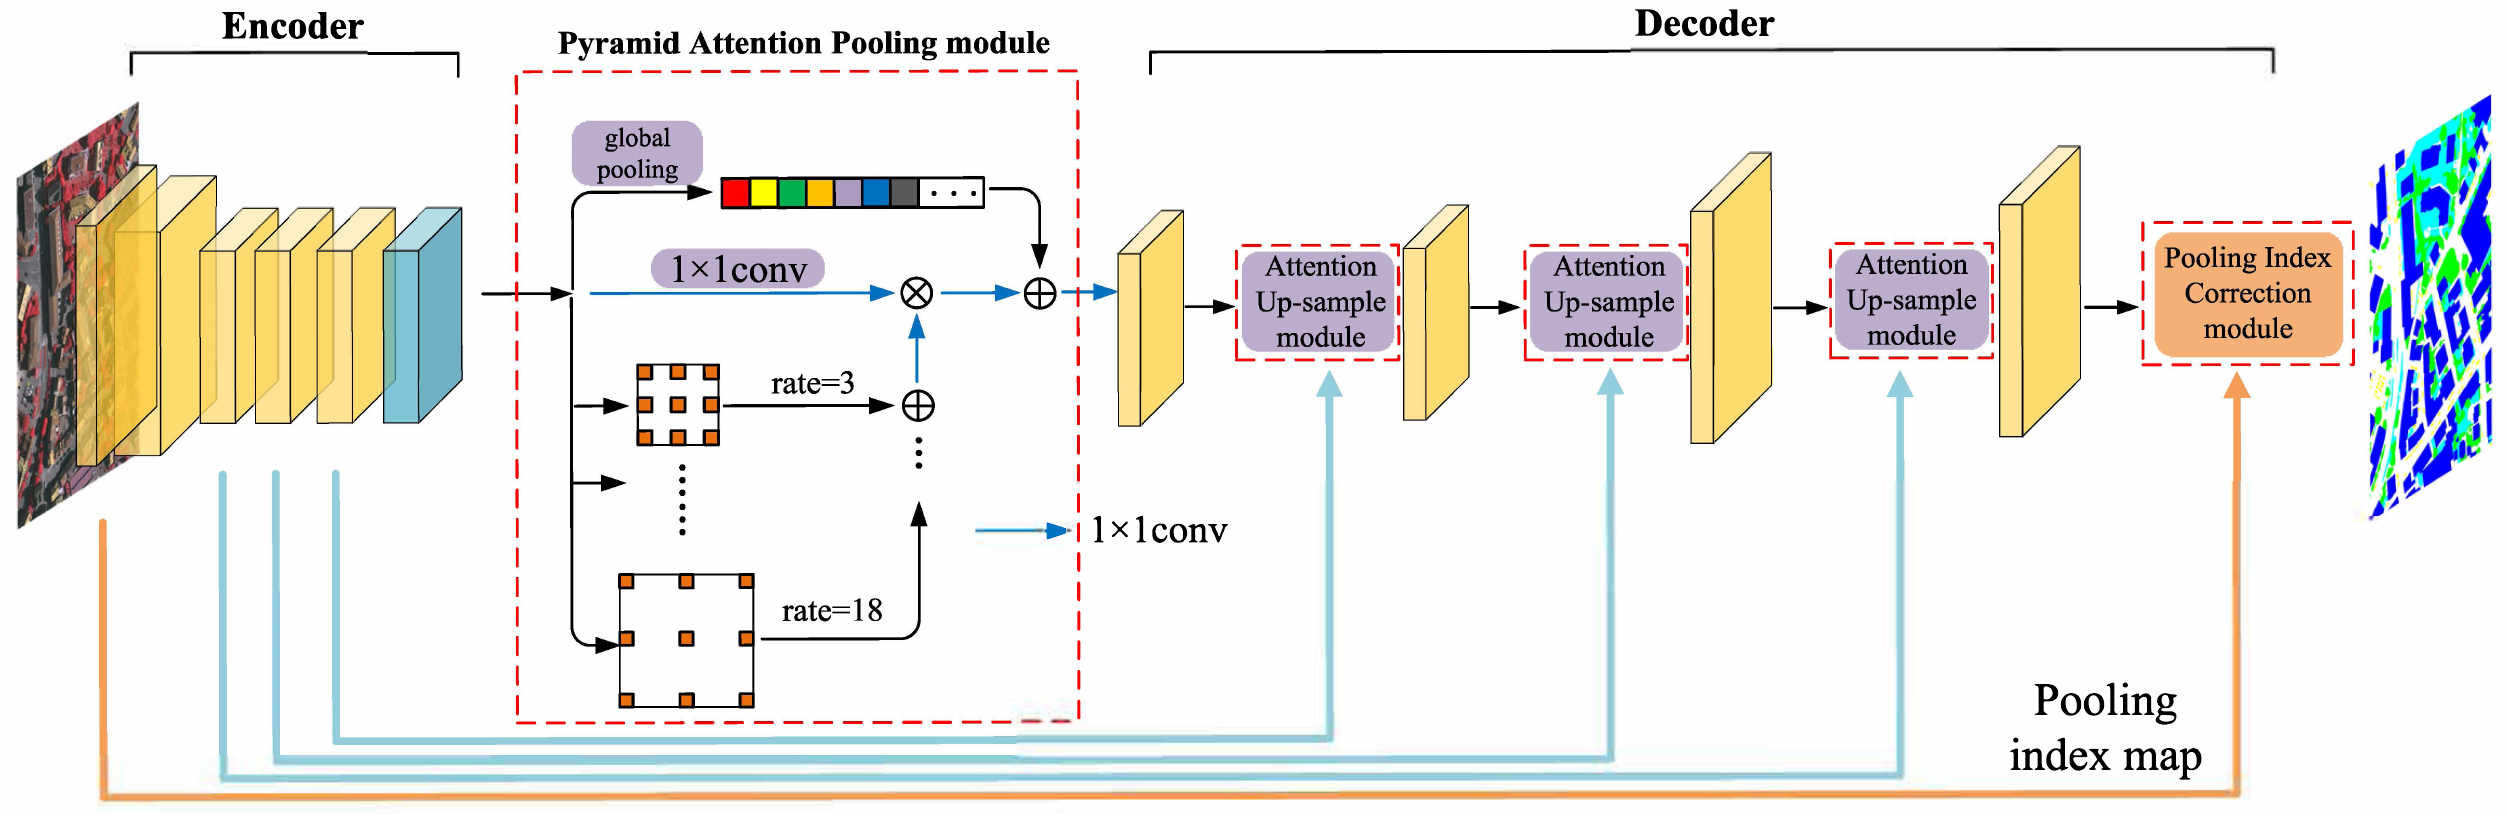
\includegraphics[width=\imgWidthXL]{images/attention_remote_sensing.png}
    \caption[Remote sensing framework]{Attention-based semantic segmentation framework for remote sensing images. Image from \cite{9513251}.}
    \label{attention_remote_sensing}
\end{figure}

\squote{MA-Unet: An improved version of Unet based on multi-scale and attention mechanism for medical image segmentation} \cite{https://doi.org/10.48550/arxiv.2012.10952} from 2020 presents MA-Unet which is an improved version of the U-Net architecture which that combines multi-scale features and attention to achieve better performance in medical image segmentation tasks. The authors propose this model to overcome the limitations of U-Net when capturing multi-scale context and addressing the imbalance between fore and background classes. The first improvement of MA-Unet is a Multi-scale Context Aggregation module designed to capture the context information at different scales. It uses a series of parallel convolutional layers with different dilation rates to help the model to learn features at several scales to improve segmentation performance. The second improvement over U-Net is a Channel Attention module and a Spatial Attention module, where the former focuses on enhancing the most relevant features in each channel and the latter focus on the most critical spatial locations, allowing the network to pay more attention to the target regions and suppress irrelevant information. The model is evaluated on the ISBI 2015 EM \cite{DBLP:conf/isbi/2015} and BraTS 2018 \cite{DBLP:journals/corr/abs-1811-02629} datasets and compared against the original U-Net and several other state-of-the-art methods. The results demonstrate that MA-Unet outperforms the other models and improves U-Net by incorporating multi-scale context and attention.

\section{Reinforcement Learning}
While some minimal concepts about \ac{RL} were already discussed in \secref{subsec:unsupervised_learning}, this section will first cover some basics about \ac{DRL} which combines deep learning and \ac{RL} and then relate it to semantic segmentation. 

The paper \squote{Deep Reinforcement Learning: An Overview} \cite{DBLP:journals/corr/Li17b} from 2017 presents an extensive overview of \ac{DRL} explaining key components, algorithms, and applications. The paper highlights the significance of \ac{DRL} and the impact it has on various fields such as robotics \cite{8675643}, healthcare \cite{8031178}, finance \cite{8701368}\cite{https://doi.org/10.48550/arxiv.2011.09607} and gaming \cite{Lample_Chaplot_2017}. The paper further provides background on \ac{RL}, deep learning, and \ac{ML} and then discusses the difference and critical algorithms of \ac{DRL} frameworks, such as value-based, policy-based, and model-based frameworks. Some key algorithms mentioned in this paper would be \acp{DQN} \cite{pmlr-v120-yang20a}, Double \acp{DQN} \cite{van_Hasselt_Guez_Silver_2016}, Dueling \acp{DQN} \cite{pmlr-v48-wangf16}, Deep Deterministic Policy Gradient \cite{DBLP:journals/corr/Casas17}, Proximal Policy Optimization \cite{DBLP:journals/corr/SchulmanWDRK17}, Trust Region Policy Optimization \cite{pmlr-v37-schulman15}, and Hindsight Experience Replay \cite{NIPS2017_453fadbd}, discussing their advantages, limitations, and improvements over traditional \ac{RL} methods.

\squote{Context-Reinforced Semantic Segmentation} \cite{Zhou_2019_CVPR} from 2019 introduces a novel Context-reinforced semantic segmentation network called CiSS-Net to improve semantic segmentation performance by leveraging context information from predicted segmentation maps. The network comprises two sub-networks called the Context Net and the Segment Net. The Context Net is designed to learn context information from the predicted segmentation maps, while the Segment Net incorporates the learned context to enhance the segmentation process. The context learning problem is designed as a Markov Decision Process with \ac{DRL} used to optimize the process. The predicted segmentation maps serve here as the environment and the Context Net as the agent. The method results in an end-to-end trainable network that achieves state-of-the-art performance on several segmentation datasets by improving the mIoU of 3.9\% over the baseline models. For further info on the architecture, see \figref{context_reinforced_sem_s}
\begin{figure}[H]%[htbp]
    \centering
    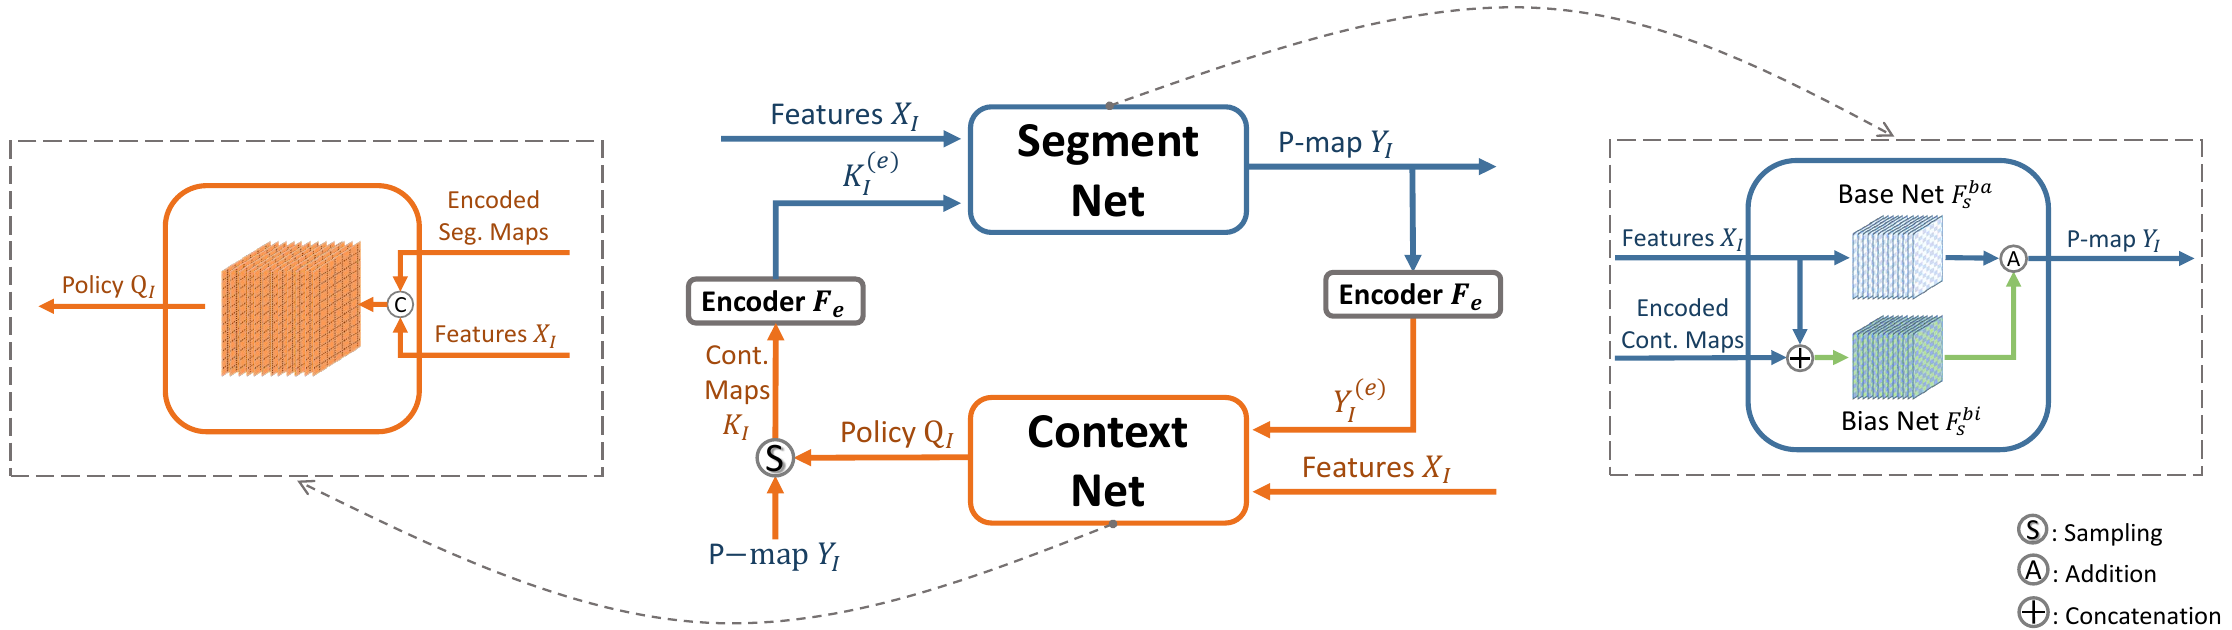
\includegraphics[width=\imgWidthXL]{images/context_reinforced_sem_s.png}
    \caption[Context-reinforced Semantic Segmentation]{The image describes the two sub-networks called Segment Net and Context Net, which mutually benefit each other and work iteratively. The Segment Net is trained based on specific context maps generated by the Context Net to improve the semantic segmentation task further. The image was taken from \cite{Zhou_2019_CVPR}.}
    \label{context_reinforced_sem_s}
\end{figure}